\documentclass[fleqn]{scrartcl}% fleqn aligns math equations to the left

\usepackage[T1]{fontenc}%
\usepackage[utf8]{inputenc}%
\usepackage{lmodern}%
\usepackage{textcomp}%
\usepackage{lastpage}%
\usepackage{parskip}%
\usepackage[letterpaper,left=0.8in, right=0.75in, top=1.0in, bottom=0.75in, includefoot, heightrounded]{geometry}%
\usepackage{graphicx}%
\usepackage{amsmath}
\usepackage[hidelinks]{hyperref}%
\usepackage{blindtext}
\usepackage[super]{natbib} % for references in superscript

% external references, as in Supplmentary Materila
\usepackage{xr}
\externaldocument[suppl]{supplement}  % `suppl' is the prefix to be used

% submission requirements in ancient journals
\usepackage{lineno} % enumerate each line
\linenumbers
\linespread{2}
%%%%%%%%%%%%%%%%%%%%%%%%%%%%%%%%%%%%%%%%%%%%



\newcommand{\etal}{\textit{\!et al.\,}}


\title{Lorem ipsum dolor sit amet}%
\author{Marcus Tullius Cicero}%
\date{\today}%
%
\begin{document}

    \maketitle
    \begin{abstract}
        A result that does not use the ``novel\("\) word in its abstract.
    \end{abstract}


    \clearpage
    \section*{Introduction}
    Marcus Tullius Cicero (3 January 106 BC – 7 December 43 BC) was a Roman statesman, lawyer, scholar, philosopher,
    writer and Academic skeptic, who tried to uphold optimate principles during the political crises that led to the
    establishment of the Roman Empire.\cite{abalem2018double}
    His extensive writings include treatises on rhetoric, philosophy and politics.
    He is considered one of Rome's greatest orators and prose stylists
    and the innovator of what became known as ``Ciceronian rhetoric''.

    \clearpage
    \section*{Methods}
    As stated in Eq.\,\ref{eq:mauris}
    \newline
    \blindtext
    % it is recommened not to use eqnarray any more, see
    % https://tex.stackexchange.com/questions/285226/is-eqnarray-really-obsolete
    \begin{align}\label{eq:mauris}
        \textnormal{Mauris lacinia}: \hspace{0.5in}	 f(a) = e^{-(a/\beta(a))^2}.
    \end{align}



    \clearpage
    \section*{Results}
    See Fig.\,\ref{fig:tullius}
    \newline
    \blindtext\,\
    See also supplementary Fig.\,S\ref{supplfig:ciceroskyrim}


    \clearpage
    \section*{Discussion}
    \blindtext

    \clearpage
    \section*{Acknowledgements}
    \blindtext

    \clearpage
    \bibliographystyle{vancouver}
    \bibliography{cicero}


    \clearpage
    \section*{Figures}

    \begin{figure}[ht]%
        % note: figure argument should not include the extension
        \centering{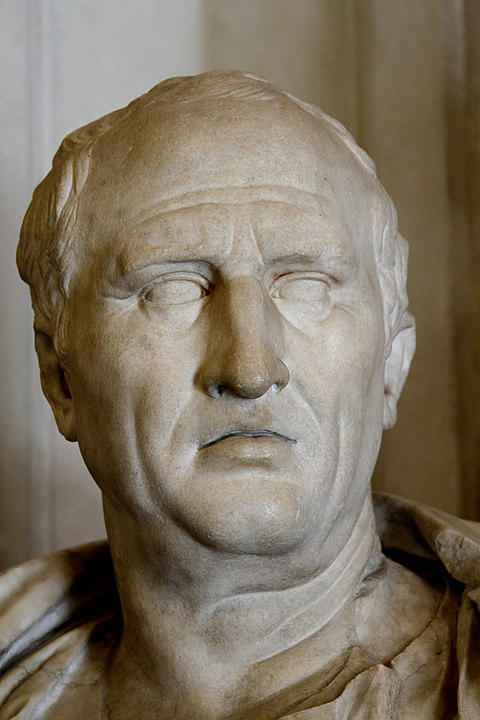
\includegraphics[width=0.5\linewidth]{figures/tullius}}
        \caption {Marcus Tullius Cicero, marble bust.}
        \label{fig:tullius}
    \end{figure}





\end{document}